\documentclass[xcolor=dvipsnames,hyperref={pdfpagelabels=false}]{beamer}

\usetheme{Boadilla}

\newcommand{\bi}{\begin{itemize}}
\newcommand{\ei}{\end{itemize}}
\newcommand{\be}{\begin{enumerate}}
\newcommand{\ee}{\end{enumerate}}
\newcommand{\bc}{\begin{center}}
\newcommand{\ec}{\end{center}}
\newcommand{\bd}{\begin{description}}
\newcommand{\ed}{\end{description}}
\newcommand{\I}{\item}
\newcommand{\f}{\frame}
\newcommand{\ft}{\frametitle}

\title{Offline Software Overview}
\subtitle{GlueX Collaboration Meeting}
\author[Mark Ito]{Mark M.\ Ito}
\date{October 9, 2015}
\institute[JLab]{Jefferson Lab}

\begin{document}

\f{\titlepage}

\f{\ft{Topics for Following Talks}
\bi
\I Offline Monitoring: Kei
\I Conversion to Geant4: Richard
\ei
}

\f{\ft{New Offline Software Wiki Page}

\begin{columns}
\begin{column}{2.0in}
\small
\be
\I General Information
\I Software Documentation
\I Offline Data Monitoring
\I Computing Facilities
\I Software Management
\I Meetings and Reviews
\I Communication and Help
\I Legacy Links
\I Uncategorized Links
\ee
\end{column}
\begin{column}{2.5in}
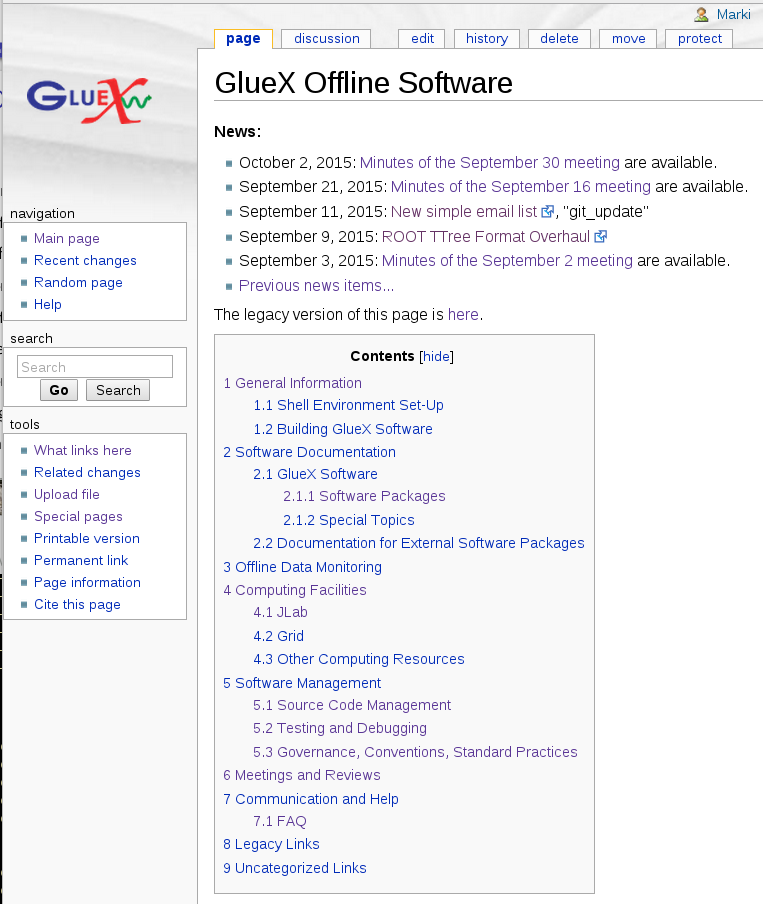
\includegraphics[width=2.4in]{offline_wiki_3.png}
\end{column}
\end{columns}
}

\f{\ft{Conversion to Git}

Director's Review of 12 GeV Software Computing, June~7-8,~2012, Committee Recommendations:

...

17.\ While we encourage the move to git as a code management system, be sure not to underestimate the extent of the paradigm shift. Identify a workflow model for your use of git. Communicate clearly the new paradigm (easy branching, no central repository, etc.). Set up (or link to) tutorials for users with a mapping of routine CVS tasks to their git equivalents (such as cvs diff, etc.). Document or link to documentation for standard git tasks without obvious equivalent in CVS or SVN, such as git rebase, or bisect.

...
}

\f{\ft{Why Change?}
  \bi
  \I Better management of changes
  \I Better communication of changes
  \I Better documentation of changes
  \I Less down-time with broken code on trunk
  \ei
}

\f{\ft{Repositories on GitHub}
  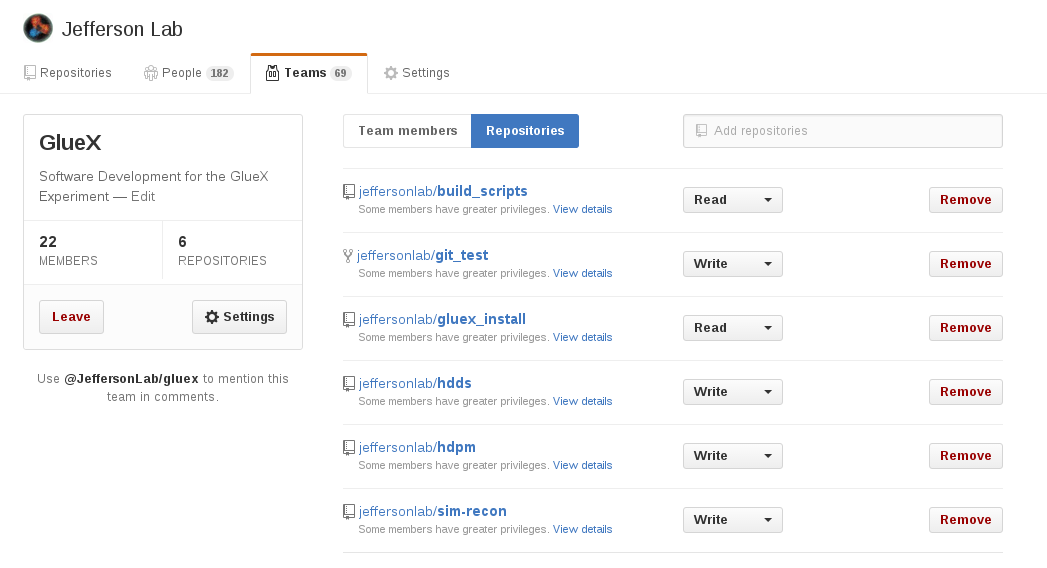
\includegraphics[width=4.5in]{repositories.png}
  }

\f{\ft{Notes on Git/GitHub}
  \bi
  \I Everyone needs an account on GitHub.
  \I Anyone can update the master branch.
  \I Changes should go onto topic branches, but enforced only administratively.
  \I Nightly builds working from the Git Repositories
  \I ``git\_update'' simple email list: daily digest of changes
  \I Team Maintainers and Team Administrators
  \ei
}

\f{\ft{Spring 2015 Simulations Complete}
\bi
\I 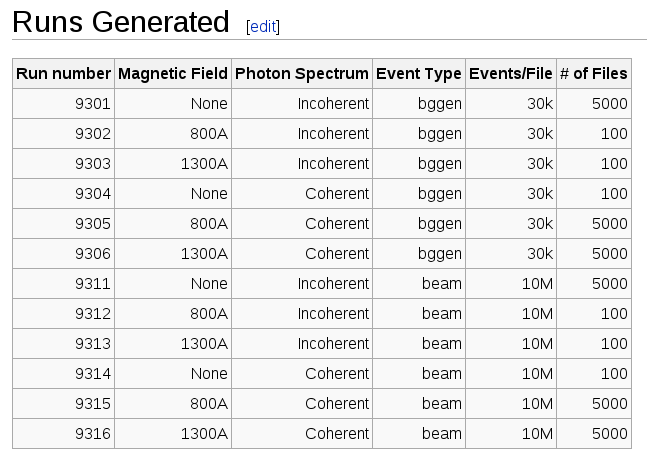
\includegraphics[width=3.5in]{spring_sim_conditions.png}
\I Used sim-recon-1.3.0
\I Run 9306 redone with sim-recon-1.5.1 (BCAL ``raw'' data generated)
\ei
}

\f{\ft{Hall D Package Manager (HDPM) from Nathan Sparks}
$$
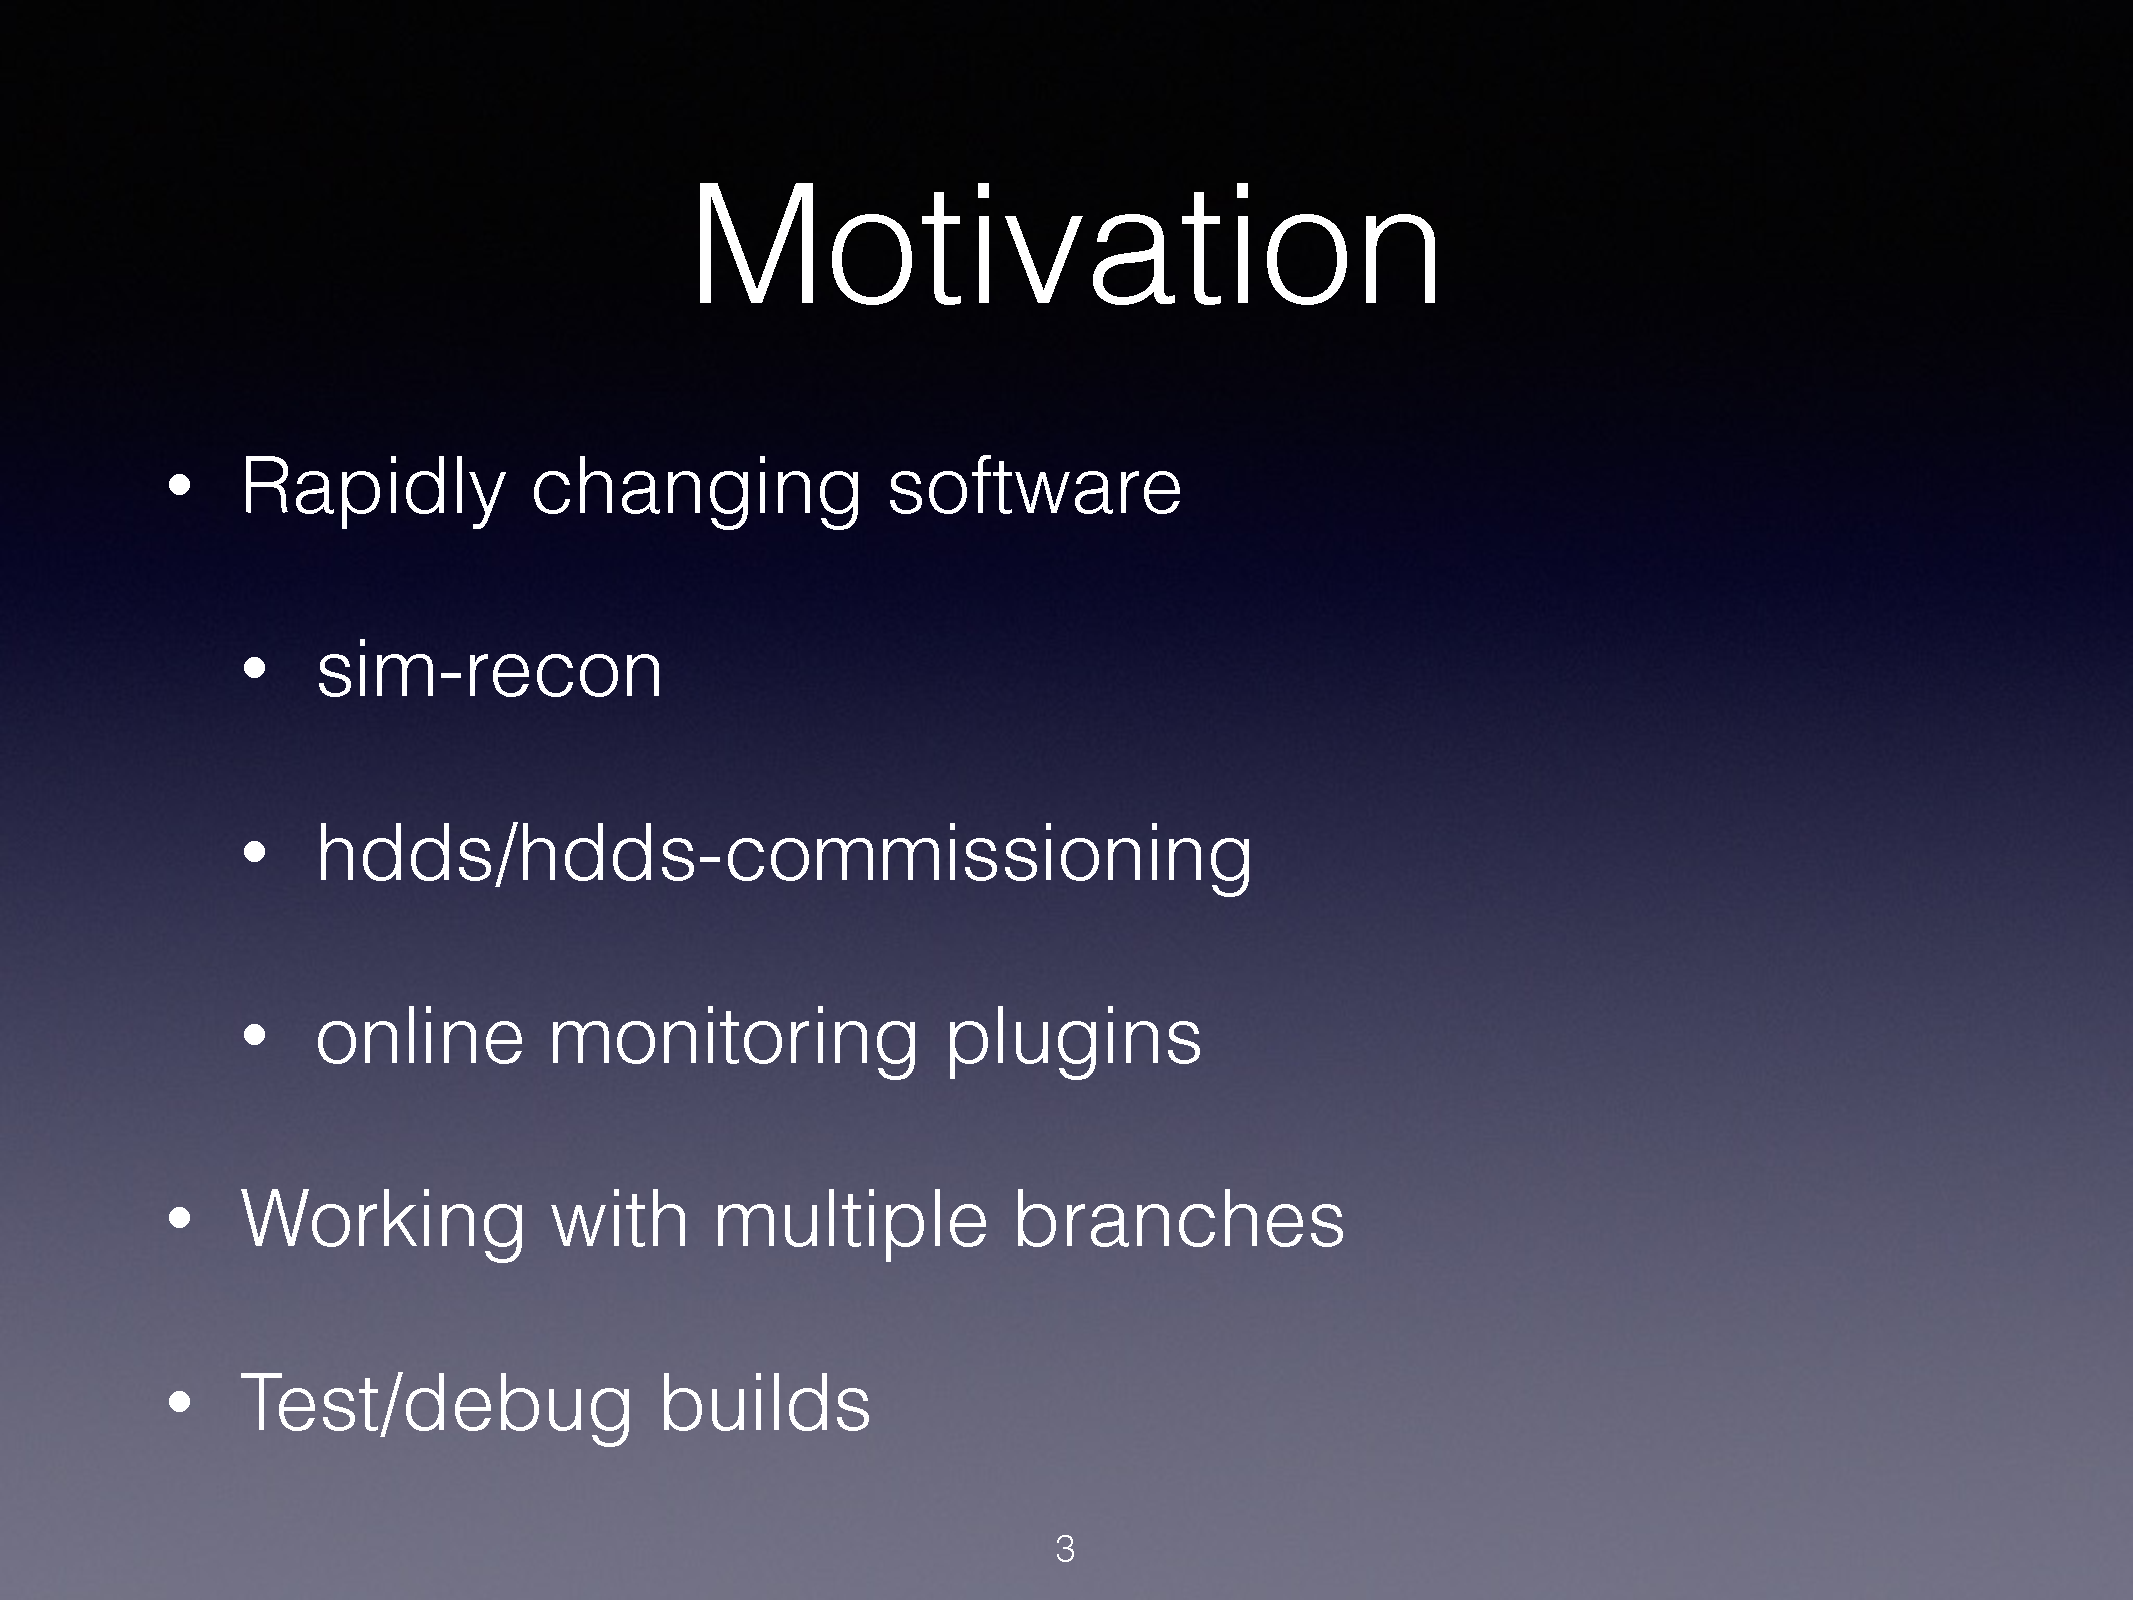
\includegraphics[width=4.0in]{hdpm_motivation.pdf}
$$}

\f{
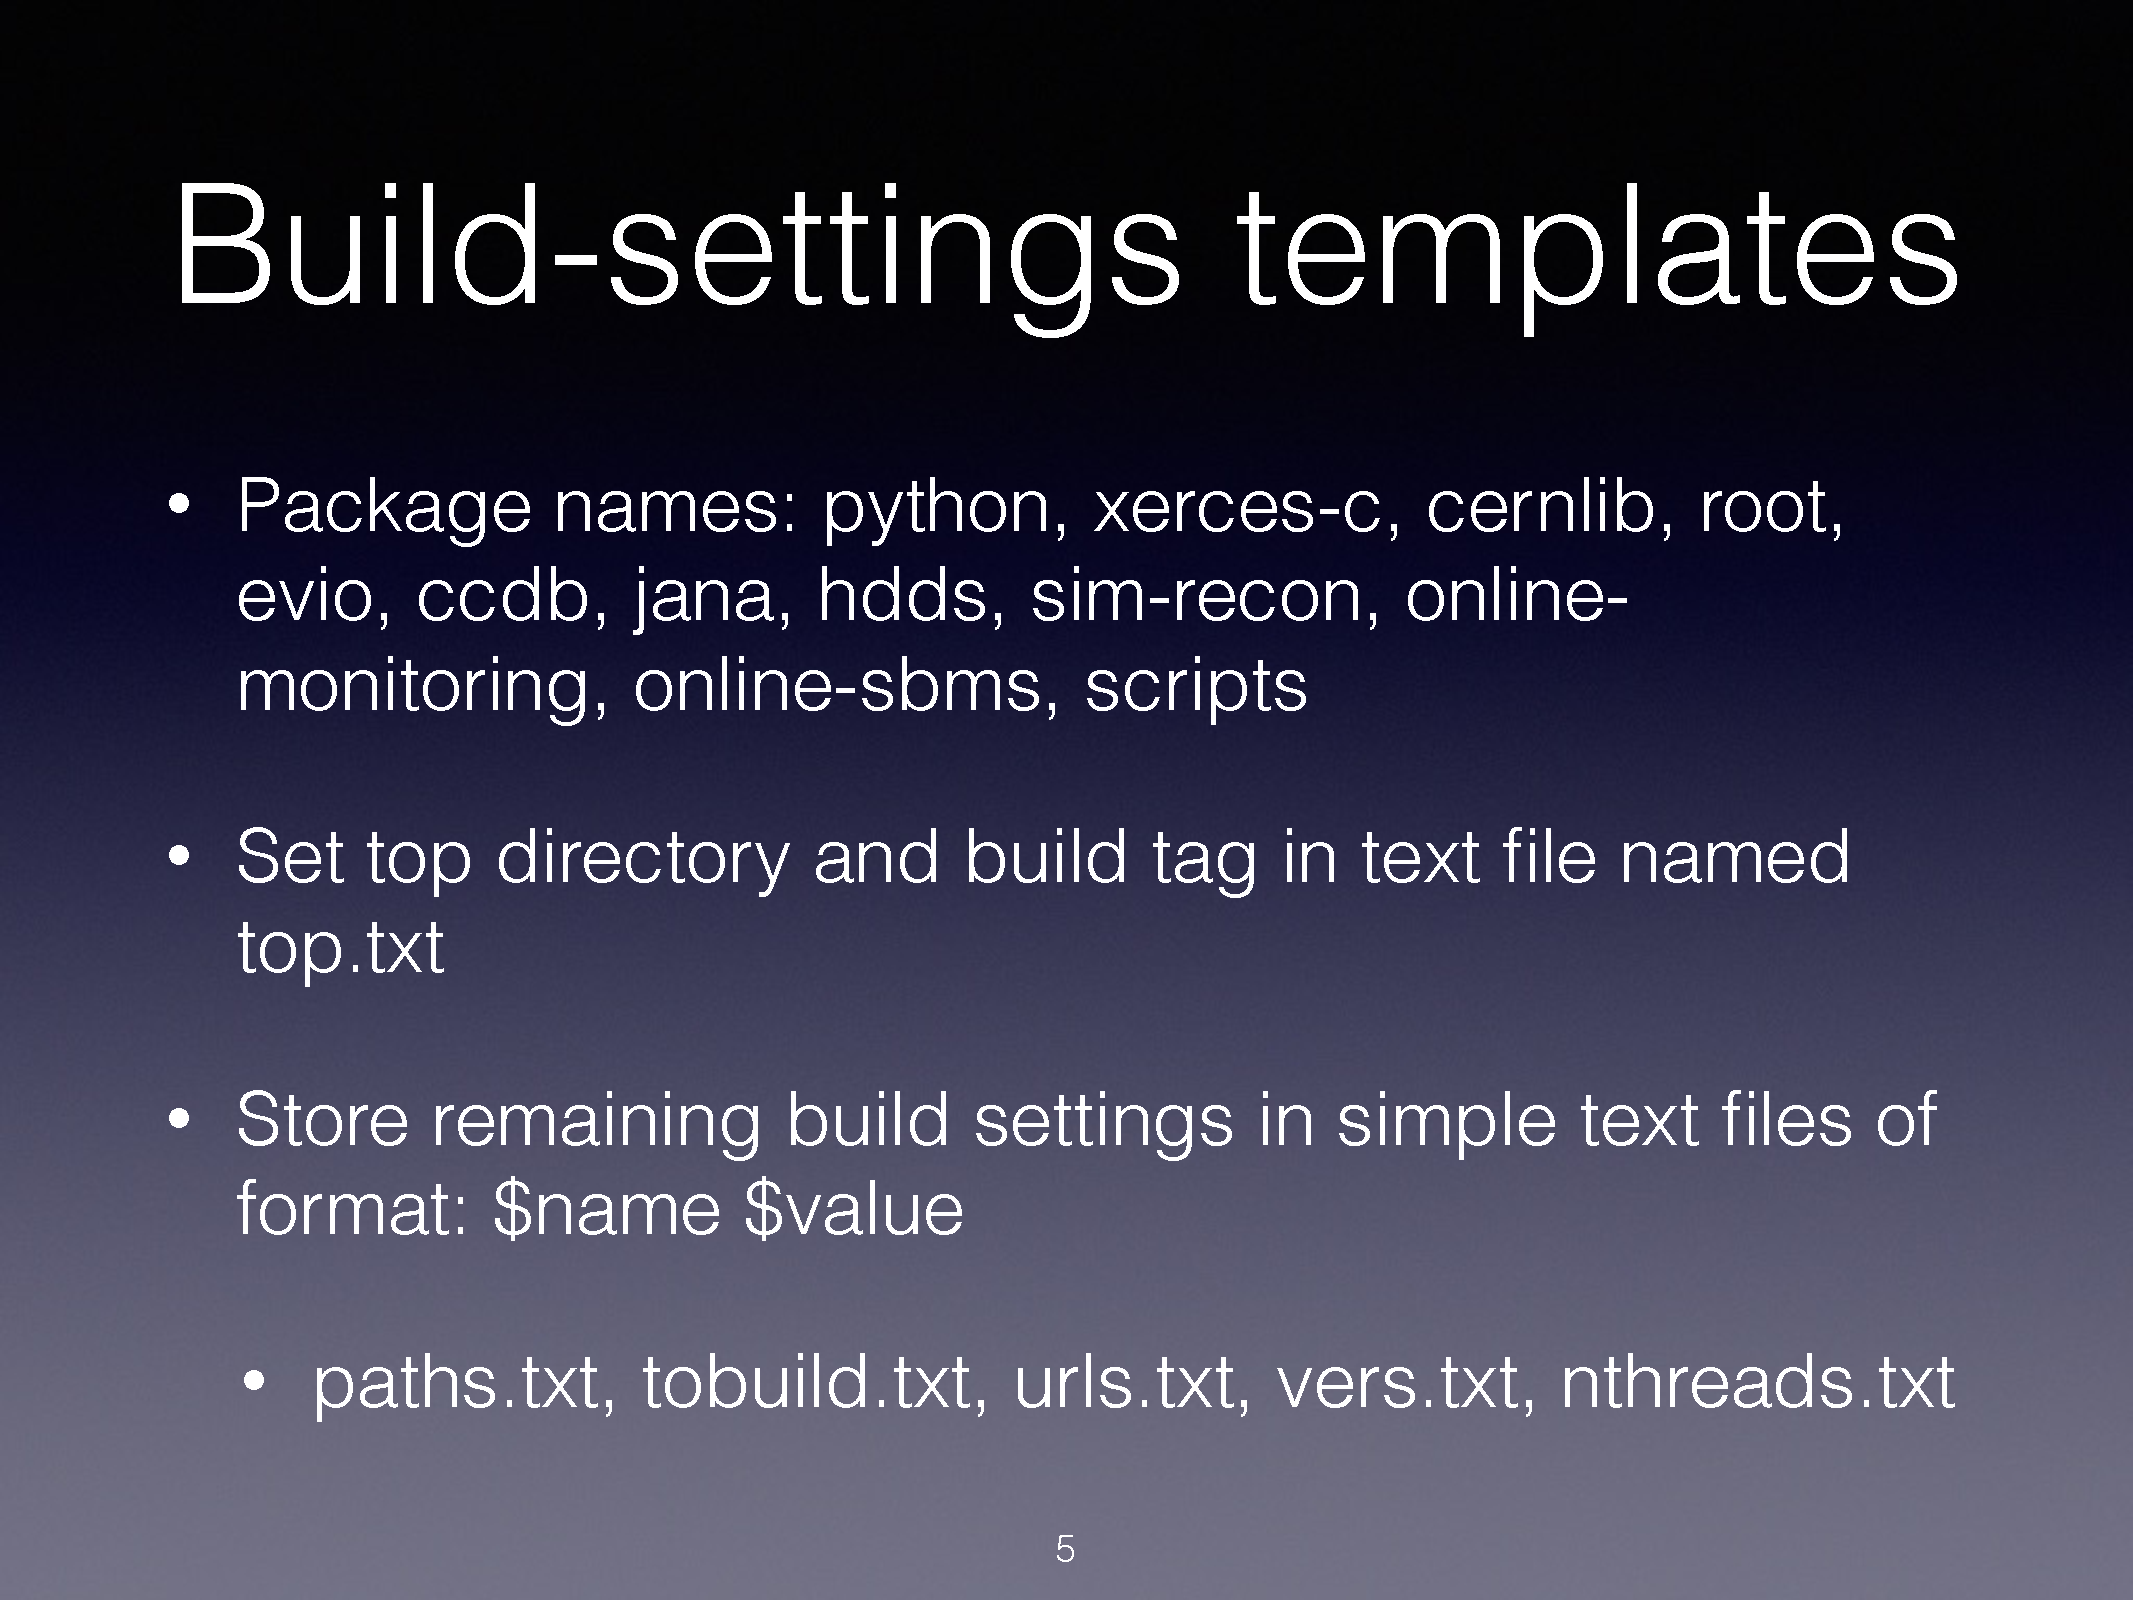
\includegraphics[width=4.5in]{hdpm_templates.pdf}
}

\begin{frame}[fragile]
\scriptsize
settings-Sp15/top.txt:
\begin{verbatim}
# top   build-tag
default Sp15
\end{verbatim}
settings-Sp15/vers.txt:
\begin{verbatim}
xerces-c  3.1.2
cernlib   2005	
root      5.34.26
evio      4.3.1
ccdb      1.05
jana      0.7.3
hdds      latest
sim-recon latest
\end{verbatim}
settings-Sp15/commands.txt:
\begin{verbatim}
hdds      "scons -u install"
sim-recon "scons -u -j8 install"
\end{verbatim}
\end{frame}

\begin{frame}[fragile]
\scriptsize
settings-Sp15/paths.txt:
\begin{verbatim}
xerces-c  /group/halld/Software/builds/[OS]/xerces-c/xerces-c-[VER]
cernlib   /group/halld/Software/builds/[OS]/cernlib
root      /group/halld/Software/builds/[OS]/root/root_[VER]
evio      /group/halld/Software/builds/[OS]/evio/evio-[VER]
ccdb      /group/halld/Software/builds/[OS]/ccdb/ccdb_[VER]
jana      /group/halld/Software/builds/[OS]/jana/jana_[VER]
hdds      hdds
sim-recon sim-recon
\end{verbatim}
settings-Sp15/urls.txt:
\begin{verbatim}
xerces-c  http://www.motorlogy.com/apache/xerces/c/3/sources/xerces-c-[VER].tar.gz
cernlib   http://www-zeuthen.desy.de/linear_collider/cernlib/new/cernlib.2005.corr.2014.04.17.tgz
root      https://root.cern.ch/download/root_v[VER].source.tar.gz
evio      https://coda.jlab.org/drupal/system/files/coda/evio/evio-4.4/evio-[VER].tgz
ccdb      https://github.com/JeffersonLab/ccdb/archive/v[VER].tar.gz
jana      https://www.jlab.org/JANA/releases/jana_[VER].tgz
hdds      https://github.com/JeffersonLab/hdds
sim-recon https://github.com/JeffersonLab/sim-recon
\end{verbatim}
\end{frame}

multi-threaded mcsmear
Mixing Simulated Events
New releases, jana, sim-recon, hdds

new volatile disk hardware
new work disk hardware
Offline style build on gluex cluster
ROOT 6
Turning the Fine-Mesh Field Map into a Resource
Moving the Plug-Ins.
Policy on CCDB Variations for Reconstructing Simulated Data (Mark)
Overhaul ROOT TTree Format (Paul)
Software for Correcting for Pedestal Drifts
Data Challenge 3 update
Default for builds: with debug symbols or without?
Fall 2015 Commissioning Simulations. 
Some problems with F125 algorithms?
Auto-Build on Pull Request
Noise Studies

\end{document}
